\hypertarget{plotting-and-transition}{%
	\midheading{Plotting routine and transition function}\label{plotting-and-transition}}

The following transition function is implemented for the example
input files. For more details we refer to our publication. The fully
matched cross-section is described in general by 

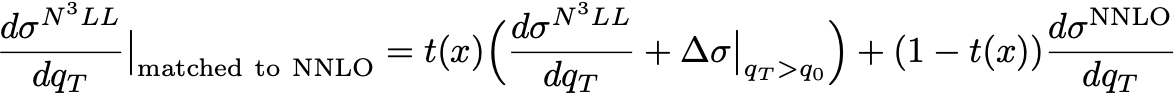
\includegraphics[width=0.9\textwidth]{./sections/Matching.png}
%\begin{equation}\label{eq:matchingmod}
%        \;
%	\left.\frac{\mathrm{d}\sigma^{\text{N$^3$LL}}}{\mathrm{d}q_T}\right|_{\text{matched to \NNLO{}}} 
%	=  t(x) \left( \frac{\mathrm{d}\sigma^{\text{N$^3$LL}}}{\mathrm{d}q_T} + 
%	\left.\Delta\sigma\right|_{q_T>q_0} \right)
%	+ (1-t(x)) \frac{\mathrm{d}\sigma^\NNLO{}}{\mathrm{d}q_T}\,
%\end{equation}

using a transition function $t(x)$. We have implemented a transition function $t$
with $x=q_T^2/Q^2$ that smoothly switches between 1 and 0 like a sigmoid function.

Following a choice in CuTe, we first define

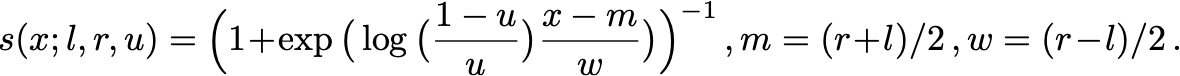
\includegraphics[width=0.9\textwidth]{./sections/sfunction.png}
%\begin{equation}
%s(x;l,r,u) = \left (1 + \exp\left(\log\left(\frac{1-u}{u}\right) \frac{x-m}{w}\right) \right )^{-1}\,,\quad
%m = (r+l)/2\,,\quad w = (r-l)/2\,.
%\end{equation}

The function $s(x)$, parametrized by $l,r,u$, is defined to be $s(l)=1-u$ and $s(r)=u$.
In terms of this sigmoid, our transition function $t(x; x^{\text{min}},x^{\text{max}},u)$, where 
$x=q_T^2/Q^2$, is then defined by
\begin{equation}\label{eq:transition}
	t(x; x^{\text{min}},x^{\text{max}},u) = \left\{\begin{array}{lr}
		1 , & \text{for } x < x^{\text{min}}\\
		\frac{s(x; x^{\text{min}}, x^{\text{max}},u)}
		     {s(x^{\text{min}}; x^{\text{min}}, x^{\text{max}},u)}, & 
		\text{otherwise}
	\end{array}\right\}\,.
\end{equation}
This ensures that below $x^{\text{min}}=(q_T^{\text{min}}/Q)^2$ only the naively matched result is 
used, and at
$x^{\text{max}}$
for small $u\ll1$ the transition function is approximately $u$. In practice it makes sense to set 
the transition
function to zero below a small threshold like $10^{-3}$ without a noticeable discontinuity.
This has the advantage that the deteriorating resummation and matching corrections do not impact 
the region of 
large $q_T$ at all.
Our example plotting routines use $x^{\text{min}}=0.001$, and $u=0.001$, and the parameter 
$x^{\text{max}}$ corresponds to the value of \texttt{transitionswitch} set in the input file. The 
transition function can be changed or completely replaced by just modifying the plotting routines. 
The following figure illustrates this transition function.

\begin{figure}[t!]
	\centering
	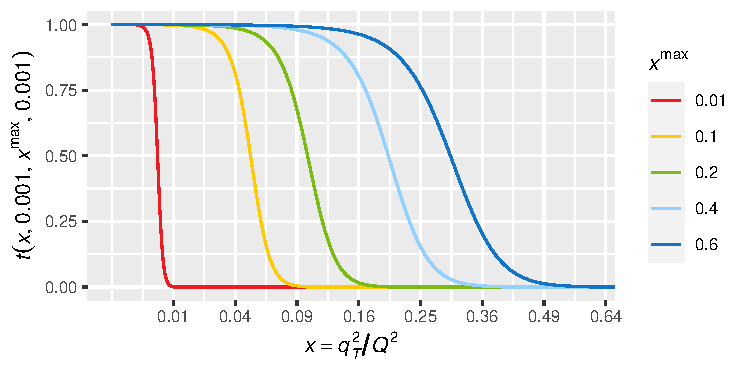
\includegraphics[width=0.8\textwidth]{transition.pdf}
	\caption{The transition function defined in eq.~\eqref{eq:transition} for different values of 
	the parameter $x^{\text{max}}$ which determines the position of the 
		transition. The $x$-axis is displayed on a square-root scale 
		to guide the eye on 
		the quadratic $q_T$-dependence.}
	\label{fig:transition}
\end{figure}
